%!TEX root = ../Thesis.tex
\chapter{Introduction to tools of supervised machine learning}

\section{Supervised machine learning to predict and to learn}
Supervised machine learning is either regression, classification or probability estimation models built on labeled data. Regression is to predict scalars (numbers), classification to predict class membership or lastly to rather predict a probability distribute across class. 

The direct motive of supervised modeling is to predict a certain target information of a given object, that is otherwise expensive/tedious to measure, or only reveal it self in the future, or the measuring is invasive and will destroy the object of interest. The target is predicted by learning a simple or perhaps complex relationship between easy accessible feature information and the target from a labeled training data set. When a useful relationship has been established with a model, target predictions can be made for a unlabeled data set without the target information.

An indirect motive of supervised machine learning is to elucidate a general relationship between features and targets. One example of an indirect motive, is when modeling the contraceptive method choice reference data set \cite{welling2016forest,lichman2013uci}. Here, +1000 Indonesian married women had answered a questioner on contraception and socio-economic status. To build a model to accurately predict contraception method choice based on 10 questions on socio-economic status was never the actual motive, as it has little practical use to ask 10 questions to only estimate one answer. Why not just ask the right question at first? However, the structure of an accurately predicting model can be an useful empiric proposal for a general relationship. What are the connections between socio-economic status and choice of contraception. Scientifically, the next step is to form testable causal link theories inspired by the captured empiric relationships.

\begin{figure}[htbp]
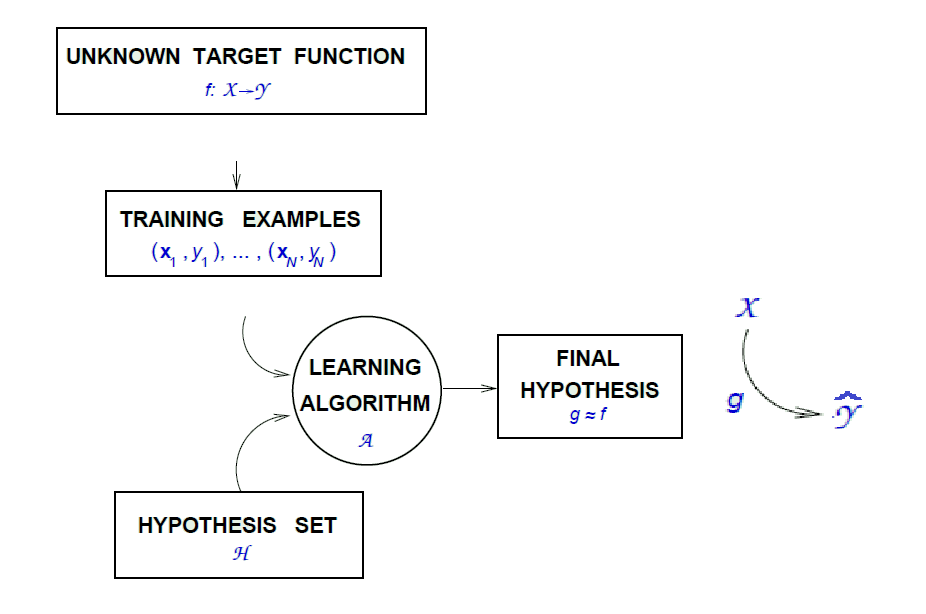
\includegraphics[width=\textwidth,height=\textheight,keepaspectratio]{graphics/sketchMLmapping.png}
\caption{We can imagine an unknown target function $f$ in nature, that generates the $N$ observed training examples $X_i$ $y_i$ for $i \in 1,2,...,N$. With a hypothesis set $H$, that is basically how we setup the learning algorithm(s) $A$, we interpret the observed examples to generate a function $g$ that mimics $f$. With $g$ we can start to predict how $f$ behaves (direct motive), or secondary evaluate the structure of $g$ to challenge both the validity of $g$ and our current beliefs of $f$.
The figure is reproduced from a set of Caltech lecture slides \cite{Mostafa13learning}.
}
\label{modelPredictExplain}
\end{figure}

A typical labeled data set, is organized as a data table with one column with desirable target information and a series of columns with feature information. Every row is an independent observation of one target and features. A practical example is the public abalone data set. Here, a marine biologist may be interested in estimating the age of abalones (shellfish). However, determining age is tedious and requires to sacrifice each specimen to study the broken shell under a microscope after chemical staining. To measure the size and weight and to observe the gender is in contrary easy \cite{lichman2013uci}. Therefore the marine biologist can use a supervised regression model to learn a relationship between morphology and age, and use the this relationship to predict effortless the age of new specimens.

\subsection{Univariate Regression}
Perhaps a single feature such as weight ($x_{.1}$) would be almost perfectly linear related to age ($y_.$). In such case uni-variate linear regression (ordinary least squares) would be a sufficient model. Where $\hat{y} = b_1 x_{.1} + b_0$, and where $b_1$ and $b_0$ are chosen to minimize a loss function evaluating the training error. Let $x_{.1}$ be a vector of weight measurements for abalone in training set and let $y_.$ be a vector target measurements, age. Both $x_.1$ and $y_.$ are of length $N$, the sample size of the training set, and the elements are enumerated from $1$ to $N^{th}$ observation by $i$, such that $y_i$ is the age of the $i^{th}$ abalone, and $x_{i1}$ is the weight.

Perhaps the abalones growth rate increases with age, and therefore the age of larger abalones are in general overestimated. By plotting the relationship and inspecting the residuals it was obvious that linear fit was not optimal. To overcome this the model may be manually expanded with a quadratic term such that $\hat{y} = b_2 x_{.1}^2 + b_1 x_{.1} + b_0$.  Thus in this manual approach, first a linear fit was made, and by inspecting the residuals it was obvious that transforming the weight measurements by non-linear quadratic transfer function would improve the linear relationship.

\subsection{Multiple linear regression and interaction terms}
The user may now start to include several transposed features and interaction terms and proceed to an extend where the number of input features in the regression model even outnumbers the number of observations. Thus there is no direct limitation in linear regression to not model non-linear relationships and interactions terms, all these terms just have to be stated manually. For a small set of features, and where the goodness-of-fit of a linear model is already fair, it is easy to inspect the residuals to observe how a linear fit may be inadequate. Hereafter one can specify some useful transfer functions and interactions terms and obtain an even better model. When the number of features become large, it will become tedious to manually state terms in the model. The individual lack of fit for a series of features to the target may blow up the residuals, making it difficult to discern what transfer functions should be chosen to each individual feature. A fast fix is to state a model with several transfer functions for each feature and interactions for each pair of features.

One limitation is the degrees of freedom. In a linear ordinary least squares model, if the number of parameters to fit in the model outnumbers the number of observations, there is no longer one unique fit with a minimal loss function score, but rather a subset of solutions all with a constant error. It takes only an offset and a slope to connect two points with a line, or an offset and two slope coefficents to describe a plane connecting three points. Likewise, 18 points can always be connected by an 17-dimensional hyper plane plus an offset.

The accuracy of a model should not be evalauted by training error, especially when then number of parameters are close to as many observations and/or if the observations are noisy.

\begin{quotation}
"With four parameters I can fit an elephant, and with five I can make him wiggle his trunk"  - J Neumann
\cite{wiki2016John}
\end{quotation}

Psychologist and economist Daniel Kahneman noted when working with notoriously noisy data from psychology tests, that multiple linear regression models explained the training data well, however the established model predicted poorly future results and could not be reproduced.
Each subject (person) would be exposed to a number of sub tests outputting score values. Each sub test was designed to be related to e.g. leadership performance by some measurable definition. With a multiple linear regression model the test scores could be combined to predict future leadership for interviewed candidates, however Kahneman preferred to simply use the summed total score as a predictor, thus giving each sub test the same weight. He found this approach more accurate and reproducible than multiple linear regression \cite{kahneman2011thinking}.

As the individual psychological tests aim to reflect the same target and these were likely linearly related (collinearity). Moreover, the psychological observations were inherently noisy and the training set size modest. This was a recipe for a poor overfitted MLR model. The best OLS fit may be spurious ratio between the sub tests, where some tests even are accredited by a negative coefficient, although having a positive linear relationship to the target.

Kahnemans practice of forcing all tests to have the same coefficient size is in practice the same as regularization, although a relatively crude version. A more elegant regularization method is the elastic net (EN). EN regression allow to do anything between classic multiple regression and a very strong regularization where all coefficient tend to have low values and equal size. Regularization tend to even the dependency on all features, unlike using only one feature greedily. Intutively, to rely more evenly on different information sources under noisy conditions will lead to more robust models. Secondly increased regularization tend to prevent finding some very specific ratio between correlated features to explain the target, but rather use the weighted average of correlated features to predict.

The elastic net coefficient estimation Elastic-net is a linear combination lasso and ridge, both estimating a squared coefficent penelization norm (L2/lambda) and a absolute sum norm (L1/alpha). L1 norm tend to drive features towards zero, and can be used for combined regularization and feature selection and is defined as 

\begin{equation}
\hat{\beta}_{Ridge}  = 	\underset{\beta}{\argmin} 
\sum_{i=1}^{N} (y_i - \hat{y})^2 + 
\sum_{j=1}^{p} \lambda(
	 \alpha       \beta_j^2 + 
    (\alpha -1) | \beta_j |
) \quad ,
\end{equation}

where $N$ is the number of observations/rows, and $\hat{y}_i$ is the $i^{th}$ prediction $\hat{y}_i = \beta_0 + \beta_{1:p} x_i.$ and $p$ is the number of features/columns \cite{friedman2001elements}. The so called $L2$ norm $\lambda \sum_{j=1}^{p} \beta_j^2$ penalizes the size of the coefficients. The $\lambda$ and $\alpha$ parameter are specified before the convex optimization searches for the set of coefficients, that achieve the lowest loss function score. The ordinary least squares fit only penalizes the sum squared residuals, wheres $lambda$ controls the overall penalization of coefficient size. $alpha$ is a value between 0 and 1. When $1$, only the sum squared coefficents is penalized (L2), whereas for $alpha=0$ only the sum of absolute coefficients is penalized (L1). Any value in between is a linear combination. Strict L2 penalization can never drive a coefficient entirely down to zero, as sqauring a small number below $1$ makes it even smaller. With the $L1$ penalization it is possible to drive coefficients down to zero, thus effectively omitting them from the model. $L1$ penalization can be used for feature selection, and is a better choice than step wise feature selection, that not will be mentioned again here(citation).

The elestic net estimator allow to introduce two types of gradual regularization driving down the effective number of parameters in the model. Elastic net can be seen as a learning algorithm $F$ that takes a training set $T$ and a set of hyper parameters $w$ ($\alpha$ and $\lambda$). The learning algorithm takes a training set and a selection of hyper paremeters (hypotheses) and output $F(T,w)->f$ the model function, such that the model function can make prediction $f(X)=\hat{y}$. The hyper parameters $\alpha$ and $\lambda$ should be chosen to obtain the lowest future prediction error and not necessarily to obtain the lowest training error, as the ordinary least squares fit do. To estimate what model will work best with future predictions cross-validation is used.

\section{cross validation}
There are infinite models that can explain a given training set perfectly. Especially a sufficient complex model, can always connect the dots in some way. In hind sight virtually anything can be explained. Cross-validation is a simulation of how well a given model will predict unseen data.

There are alternatives to cross-validation such as the 'Akaike information criterion' which will weight training set prediction accuracy against a penalty for model complexity. However the Akaike information criterion do not translate well to non-linear algorithmic models where the effective degrees of freedom is difficult to estimate. (citation neeeded)

Cross-validation is performed for two purposes. First, model selection, that is to compare our set of hypotheses to choose the most promising approach. In practice that is to select the most useful learning algorithm and optimize the hyper parameters and perhaps perform some feature selection. Secondly, model assessment, for a given built model structure $f$, to estimate the prediction error for unseen data generated by the same underlying function $g$ as the training set were. \cite{friedman2001elements}.

\subsection{Segregation}
The simplest cross-validation scheme is segregation. The data set of data examples is randomly divided into e.g. 50\% training observations, 25\% validation (aka. calibration) and 25\% test observations. The model parameters is estimated on the training set, the validation set is used to choose and calibrate the learning algorithm and the test set is used to estimate the future prediction error \cite{friedman2001elements}.

\subsection{Unbiased estimation}
\label{unbiased_estimation}
To perform model selection and to estimate prediction error is often the same procedure. However, especially if the set of model hypotheses is large, there may be some hypotheses, that by primarily by lead to models that explained the validation set well, selecting hypothesis with lowest validation error may be the best strategy. However, the low validation error of this hypothesis is the inseparable combination of skill plus luck. Where the skill component remains, the luck component is inherently non reproducible and will regress towards the mean \cite{kahneman2011thinking}. Thus, we don't know exactly why a given hypotheses turned out the best when evaluated on the validation set, but in average if we are to test the hypothesis on a new set of unseen data, the test set, the hypothesis would perform in worse in average than on the validation set. For models with little explained variance evaluating many hypotheses, we should expect the luck component to be substantial. The \textit{Gamblers fallacy} and the \textit{Infinite monkeys theorem} would be the extreme cases, where there is no skill and only luck. In a room of infinite monkeys typing randomly on type writers, one monkey will eventually write the complete works of Shakespeare. Would you hire this monkey expecting it to write more brilliant works in the future? \cite{wiki:gamblers,monkeys}

This problem is very related to family-wise error of multiple hypotheses testing in classical statistics and e.g. the Tukey and Bonferoni corrections. However no such corrections exists for general machine learning.

In conclusion when ever making a model selection or a parameter estimation based on a set of data, the same data set cannot for certain provide an unbiased estimation of the model performance. A new cross-validation must be wrapped around the current procedure. Lastly also within machine learning publication bias inevitably exists. An article including a model procedure with a good final test score, is more likely to be submitted and accepted. But as a component of luck may have had an influence, the published test set performances, will in average regress towards the mean, if the study were to be reproduced. Thus paradoxically, the test score is valuable as an unbiased estimation of the future model prediction error. However if we act on this test score, it is no longer unbiased. How can a test score be valuable, if we cannot use the information? This is an obvious conflict of interest, should a researcher publish the model with a better test score, or ideally with the most unbiased test score. The Kaggle machine laerning competions offers a good solution to resolve the conflict of interest. Here an extra an final test set will only be revealed after the competition is over. Each competitor now only have to focus on building the best model. Cross-validation will be used, but only to guide the competitor to make the optimal choices. If the competitor produces over optimistic internal cross validation, then she is only cheating her self \cite{seroussi2015steps}.

\subsection{Independent and identical sampling}
Any prediction error estimation from a cross-validation is based on the assumption of independent and identical sampling. Returning to Figure \ref{modelPredictExplain}, it assumed that that the distribution of training examples, test examples and future examples to predict are identical distributed. That is that $X_{test}$ and $X_{future}$ are drawn from the same larger $X_{all}$ distribution. Also, the sampling procedure recording a sequence of observations must be independent. E.g. if there is a strong auto-correlation with a oscillation interval larger than the sample size, a sample average may not be very close to the population average, as all observations happend to be recorded in a e.g. a sampling period with only observations above average.

\subsection{Transient or constant underlying systems}
Typically, cross-validation also assumes that the underlying true function $g$, see Figure \ref{modelPredictExplain} remains unchanged. When the underlying true function is a physical rule of nature, no drift is expected. However if the underlying function is drifting, the expected prediction error are probably over optimistic. Within economics, this problem is known as the Lucas Critique \cite{wiki:Lucus}. It is naive to believe economical models successful can predict future events from historical data. In a developing society events will be unprecedented due to new technology and social constructs. The rules of the game are simply changing too fast. To some extend modeling strategies in transient systems, can be validated with 'back-testing', which is a cross-validation over time testing an online learning system.

It can be difficult to decide if new observation diverge from the predicted, due to noise or  a drift an the underlying system $g$, that generates the observed targets $y$ as a function of $X$. If one expects the underlying system to be both transient and noisy, it is a tough situation. Any small training sample will have a substantial sampling error, and any large sample will be sampled across a period where the underlying function $g$ already have drifted.

\subsection{Defining training error and prediction}
The estimated training or prediction error need a loss function to score how much different the prediction is to the true target. Also when all predictions have been scored, an aggregation method is needed summarize the expected performance. Typically the average is used as aggregation method, and for regression, squared residuals is used as the loss function. Therefore, the prediction error is $err = \frac 1 N \sum_{i=1}^N L(y_i,\hat{f}(x_i)) $ where $i$ iterates a set of observations and where the squared difference  $L(a,b) = (a-b)^2$ is the loss function. Both for regression and classification it is worth to consider what aggregation rule and loss function to use, such that the trained model becomes the most useful. E.g. if a forecaster is financially penalized proportional to the sum the forecast errors, then the loss function should certainly also be absolute error $L(a,b) = |a-b|$. If the forecaster will be fired if any prediction is worse than a certain margin, one may choose only to summarize the top or bottom outliers to focus on reducing these. Also the prediction error may be far from constant across the feature space $X$, and therefore would an unconditional aggregate, such as averaging be a crude estimate. Instead the prediction error for each prediction of $X_i$ should be estimated by a error function $f_e$, such that $X_i$ $err_{X_i} = E[L(y_i,\hat{y}_i)|X_i] = f_e(X_i)$. For classification the loss function should reflect the actual cost of false positives / false negatives to maximize a reward. Classification problems can be redefined as probability estimation problems, applying a proper score rule as loss function. Probability estimation is a more elegant way to maximize a defined reward, than classification. Classification can only apply one fixed threshold of certainty, when assigning predicted classes to test observations \cite{harrell1984regression}. At best the model selection and test could be based on a simulation reflecting, what would happen if the predictions were utilized. This is known from back-testing e.g. stock trading robots. The robot will e.g. provide predictions of the coming days prize fluctuations for a year, and a trading simulation will measure how a given strategy can utilize these prediction to increase portfolio net worth and to minimize the risk (variance). Then the loss function and aggregation method is coupled to exactly, what the user intend to achieve. However, it may be difficult to estimate the outcome of good and poor predictions, when in opposite to stock trading the rules of the game is unknown. How the accuracy of the predictions of permeation enhancers provided in this thesis will affect the company Novo Nordisk is really hard to say, and therefore it is difficult to devise a test metric that optimizes wealth or happiness. A good guess would be, that most often the permeation enhancer predictions will mean nothing at all and for rare wild cards, a whole lot. This is based on the notion that most candidates in drug development will fail, and only few candidates will drive the revenue.

\subsection{n-fold cross validation, repeated validation and grid search}
some line of this

\cite{krstajic2014cross}

\section{Algorithmic models}
So far multiple linear regression have worked well even for non-linear problems, if the user can come up with transfer functions that make the feature relate linearly to the target. However, for multivariate data set, where an initial multiple linear regression model has a low goodness-of-fit, it can be difficult to decide from residuals plots by each variable, what series of transfer function and interaction terms would improve the model. Algorithmic models are loosly termed as defined as model structures rather defined by the algorithm, than the output mathematical expressions. However, model can ultimately be expressed in a mathematical expression, it may just be a very long and incomprehensible one. Popular algorithm models presently are radial basis support vector machine (RB-SVM), random forest (RF), gradient boosting trees (GBT) and neural nets (NN). An introduction to each type of model is beyond the scope of this thesis and especially neural nets has today a large field special tailored for the purpose sub-models, such as convolutional nets, recurrent nets, deep layered nets or any combination of these. 

From a users view point, all these algorithmic learners have in common that features can be inputted without specifying transfer functions, and resulting model will to some extend automatically: Fit non-linear relationships, fit interactions and provide regularization plus robustness to outliers. A given algorithmic models should be considered instead, whenever this seem to out perform linear regression in cross-validated prediction error.

In ordinary least squares, there are no hyper parameters, only one fit with the lowest training error. In the elastic net fit, $\lambda$ and $\alpha$ could be adjusted and for each set of these hyper parameters named $w$, there would be a solution of parameters / coefficients. In contrary to linaer regression, the model parameters to fit, are not necessarily stated in advance, new ones can be created in the fitting process. Each algorithmic laerner will have a set hyper parameters, and if these are calibrated poorly, the resulting model fit will be inferior.

From a user perspective, the random forest, algorithm often perform quite well with the one default set of hyper parameters, whereas GBT have no recommended default set of hyper parameters, but likely there is a smaller subset of hyper parameters that do perform better than random forest. From a user perspective, GBT can provide a slightly improved performance on the expense of application time and run time. In order to calibrate the GBT learner well, for a given data set, it likely necessary to perform a substantial grid search and thus in fact run the learner algorithm several times. With formalized grid search and cross-validation tools such as caret package, few extra lines of code are required \cite{kuhn2015short}.

The random forest algorithm was extensively used throughout this thesis. Probably either of above mentioned methods RBF-SVM, GBT and some version NN, could have replaced random forest. However the prediction error difference, may be so small, that it only in competitions, would matter which one to pick. In a competition situation, one may also choose to use all the learner algorithm and combine several trained models in a joint ensemble. 

Although the trained models are stated differently, a good rule of thumb is, that when the various models achieve very comparable cross-validation their effective model structures must match. In appendix \textit{favorite answers on cross validated}, there is included my answer to a stack-exchange question, illustrating how similar a good RF and RBF-SVM fit are for interpolation. However when then RF and RBF-SVM model is used for extrapolation outside the proximity of training observations, the model structures heavily disagree. Figure \ref{svmVSrf} depicts how similar the effective model structures are in proximity to data points, and how different extrapolated predictions are.

\begin{figure}[!htbp]
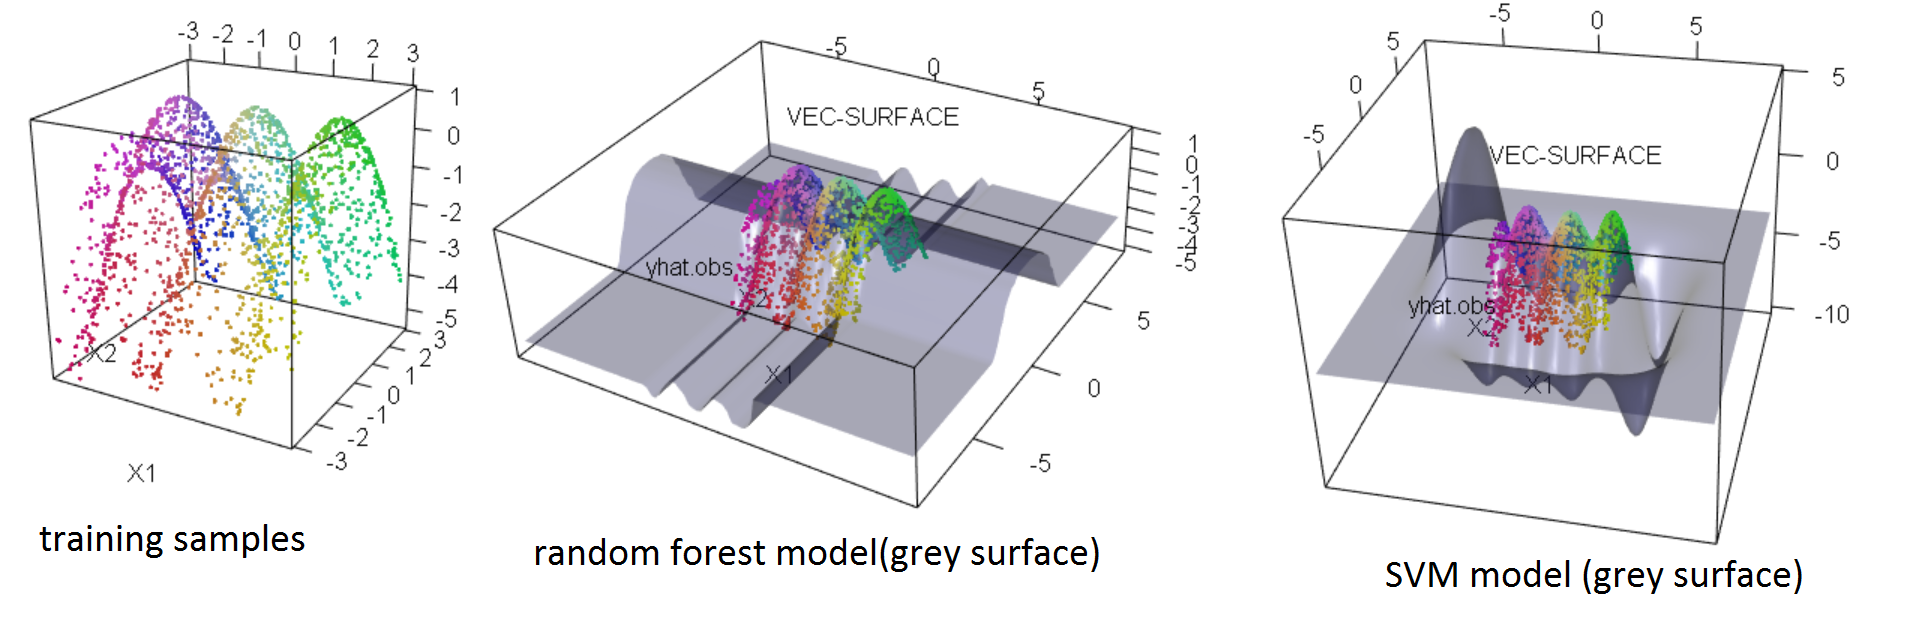
\includegraphics[width=\textwidth,height=\textheight,keepaspectratio]{graphics/svmVSrf.png}
\caption{Left plot: A training set has been simulated from  $y = sin(x1 \pi) − \frac 1 2 x_2^2$ where $x_1$ and $x_2$ are drawn from a uniform distribution within $[-3;3]$. Middle and left plot, repectively RF and RBF-SVM has been trained on the data set providing two completely similar model structures within the proximity of training data. However outside (grey surface) the RF and RBF-SVM built model structures heavily disagree. See appendix for code example.}
\label{svmVSrf}
\end{figure}


\section{random forest}

\subsection{bagging}
Random forest is a bootstrap aggregated ensemble model meaning it is collection of independently trained sub models, where each model is trained on bootstrapped sample of the training set. The prediction error of bagged ensemble models can be lower than the average prediction error of the individual models.

Bootstrapping the training set means to sample a random set of observations. This bootstrap set, can be as a large training set, however by default (uniform distribution) the chance an observation is not included is approximately 37\% spending on size of traning set. The chance an observation sampled at least once is \%63, see Appendix \ref{CV9_RFsampling) for a exact sampling description.

For random forest the same learner, decision tree, is bagged perhaps 500 times. The ensemble prediction is typically the average vote of the ensemble. Besides random forest, bagging is an easy way to combine different model approaches to achieve a perhaps lower prediction than any model approach alone. As bagging independently train each model, the computation can easily be distributed across multiple CPUs or nodes in a server cluster. Appendix \ref{CV8_combineBagging} provides an elaborate parallel implemented example, where logistic regression is combined with random forest to form a new and more accurate ensemble.

When bagging multiple linear regression models (only), the acquired ensemble can actually be reduced to one linear regression model where each coefficient is the average of the corresponding coefficient in each sub model. Hereby bagging provide a regularized model similar to increasing the $lambda$-parameter of elastic net and where $alpha=1$. For ensembles of non-linear models, there are no obvious average model (if any), that provide the same predictions. However the bagging still provide regularization offering a more robust model estimation, than a single learner model alone.


\subsection{Introduction to decision trees}
The random forest algorithm is an improvement of the classification and regression tree algorithm (CART) \cite{breiman1984classification,breiman2001random}. Overall the CART decision trees are built by applying 3 rules recursively

Rule 1: A collection of observations is called a node and a node has a prediction, the average target.

Rule 2: If a node has more than a lower limit of observations, it will be split into two nodes. A split rule is defined by a break point for given numeric features, where any observation having a feature value below or equal is forwarded to a left daughter node and otherwise to a right daughter node. Every possible split will be tried. For categorical features, any unique separation categories into to daughter nodes will be tried.

Rule 3: A loss function evaluates and select the best split, that is sum of squared residuals for regression and a variation of gini-gain for classification. See appendix for actual definition of the loss function. The regression loss function chose the split, maximize the variance across daughter nodes and minimize intra-daughter node variance. The classification loss function chose the split that produces two nodes most unlike a uniform class distribution.

Rule 4: If a node cannot be split, either as there is no valid feature left to split by or if the node do not meet the splitting criteria, the node is terminal, otherwise repeat rule 1-4 for every sub node.

Below is the Figure \ref{simpleTree}, that depicts how a tree is built. For a CART tree, the training set and root node is the same, as all observations is used to build the tree. For multiple trees random forest in a random forest ensemble, all trees share the same training set. The training observations passed to each root node of each tree is a bootstrap of the training set.

\begin{figure}[!htbp]
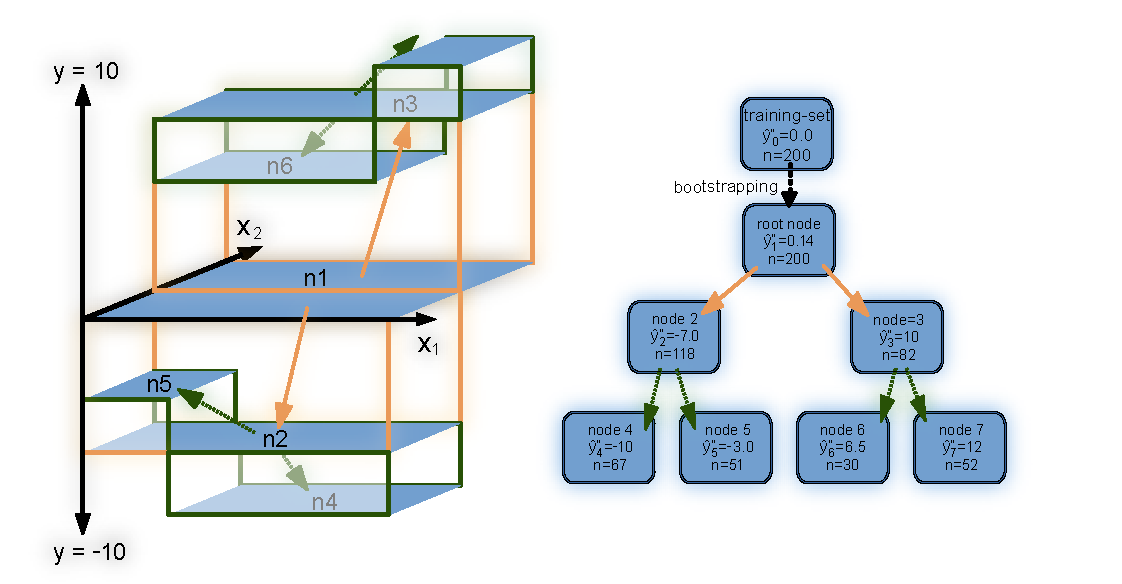
\includegraphics[width=\textwidth,height=\textheight,keepaspectratio]{graphics/randomForest_explained_thesisVersion.pdf}
\caption{somthing about trees \cite{welling2016forest}}
\label{simpleTree}
\end{figure}


Controlling parameters of the bootstrap process increase regularization and decrease the prediction error if the data is noisy \cite{welling2016forestFloor}.

Bagging ensembles
Random variable subspace \cite{ho1998random}

Something more about random forests

Leo Breiman, hyper reacntangle proof that predictions converge with infinite trees
		     



